\documentclass[a4paper]{article}

\usepackage[english]{babel}
\usepackage[utf8x]{inputenc}
\usepackage{amsmath}
\usepackage{graphicx}
\usepackage[colorinlistoftodos]{todonotes}
\usepackage[margin=1in]{geometry}
\setlength{\parindent}{0pt}
\usepackage{url}
\usepackage{float}
\usepackage[section]{placeins}
 

\title{Fourier Feature Extraction}

\author{Benjamin Goss}

\date{\today}

\begin{document}

\pagenumbering{gobble}

\maketitle


\section{Introduction}
There are many reasons that a Fourier Feature Extraction can be used on a dataset, but one of these is in order to classify letters from an input, on a smartphone or a tablet. The classifier that is shown within this report is to classify three letters, an S, a T and a V. 
\section{Analysing the Images}
In order to create the classifier, the first step that must be taken is to find the features that will be used by the classifier. The method used to complete this task is using the Fourier space to pick them out. The first thing that must be done to do this is to transform the images in to the frequency domain. This is done using a Fourier Transform. Then, the features that will be used by the classifier must be extracted from this.
\subsection{Fourier Transform}
The Fourier Transform is used to manipulate the image into an easier format to find features from. It transforms the data from the spatial domain to the frequency domain, and represents the data as sines and cosines \cite{FFT}. The equation that is used to complete the two dimensional fast Fourier Transform, which is the way that the letters are transformed to the Fourier Domain, is shown in the equation below. %insert fourier equation here
\begin{displaymath} F(u,v) = \frac{1}{MN}\sum\limits_{x=0}^M\sum\limits_{y=0}^Nf(x,y)e^{(j2\pi(ux/M+vy/N))}\end{displaymath}
The Fourier Domain shows the change in frequency of the image, with each point showing a frequency. The frequencies are in terms of real and imaginary numbers, so in order to do calculations with them, the magnitude must first be found. 
%Fourier Transform images of s t and v
\begin{figure}[H]
\centering
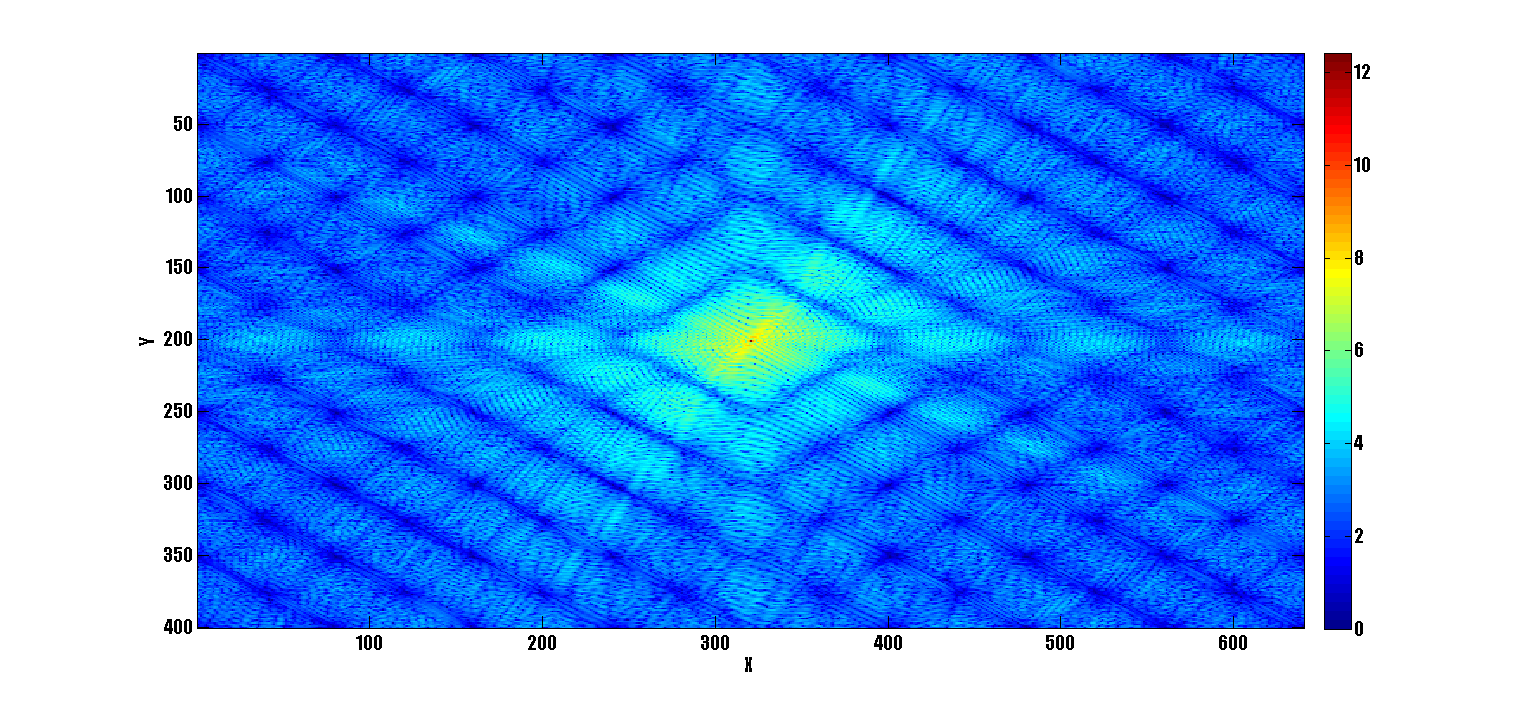
\includegraphics[width=0.5\textwidth]{plotS.png}
\caption{\label{fig:plotS}A Plot of the letter S in the Fourier Space. The lines of the S can be seen in the different frequencies.}
\end{figure}
\begin{figure}[H]
\centering
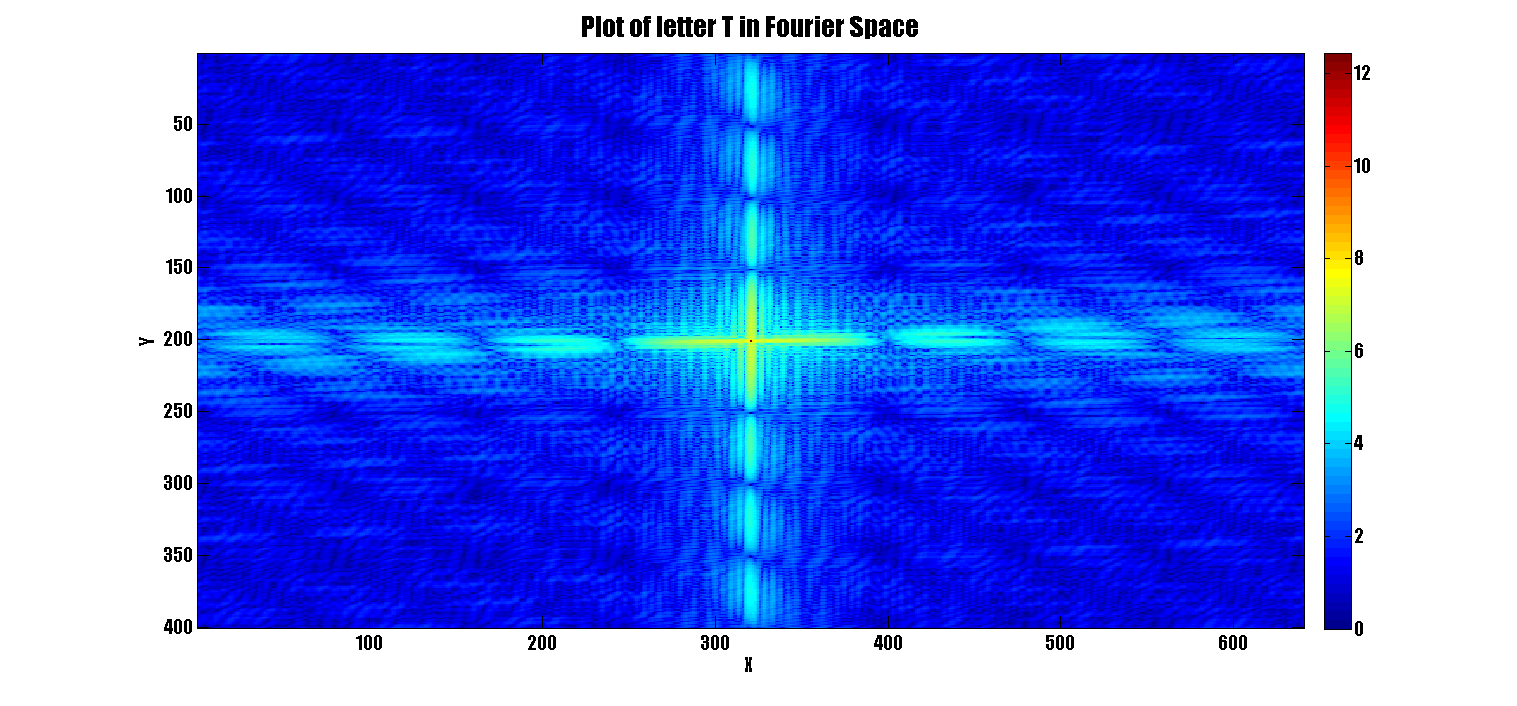
\includegraphics[width=0.5\textwidth]{plotT.png}
\caption{\label{fig:plotT}A Plot of the letter T in the Fourier Space. The lines of the S can be seen in the different frequencies.}
\end{figure}
\begin{figure}[H]
\centering
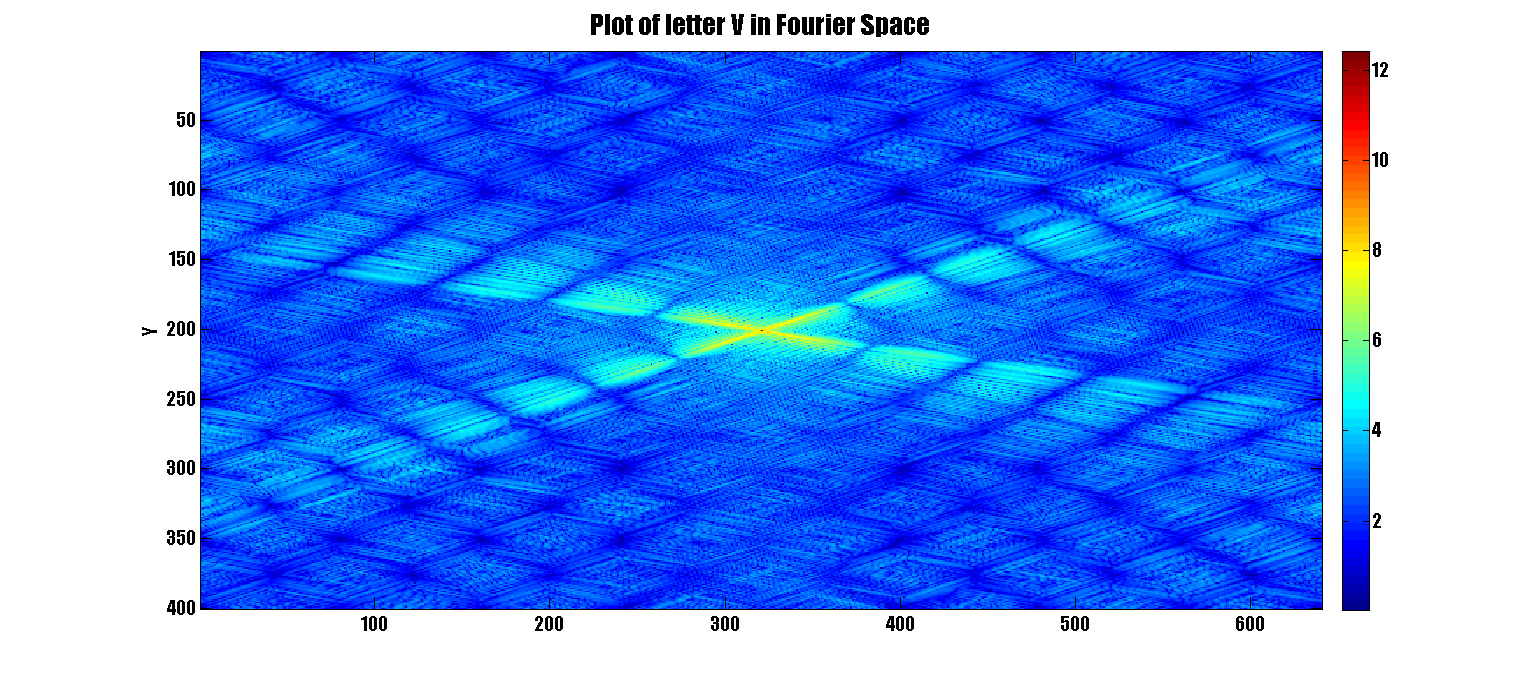
\includegraphics[width=0.5\textwidth]{plotV.png}
\caption{\label{fig:plotV}A Plot of the letter V in the Fourier Space. The lines of the S can be seen in the different frequencies.}
\end{figure}

As can be seen from Figure \ref{fig:plotT}, the vertical and horizontal lines of the T are shown in the graph. The diagonal lines of the V are also shown in Figure \ref{fig:plotV}. Figure \ref{fig:plotS} shows the various lines that are within the S, with a diagonal box shape within the graph. 
\subsection{Feature Extraction}
%Explain why you choose features
The reason features are chosen from the Fourier space is that there needs to be a way to show the differences between the objects that are to be classified. Each feature is created by choosing a section from the Fourier Space, and condensing it down to a single point. Before choosing which features to use to classify the specified letters, it was first necessary to decide how many features would be extracted. It was chosen that two features were to be picked, as it makes it easier to perform further analysis on the classifier when the features can be plotted against each other on a normal scatter graph. 
To create the features, a section of the graph is selected, and then the magnitude of that section is summed up to a single point, and that point is plotted against the point from the other selected feature.
\begin{figure}[H]
\centering
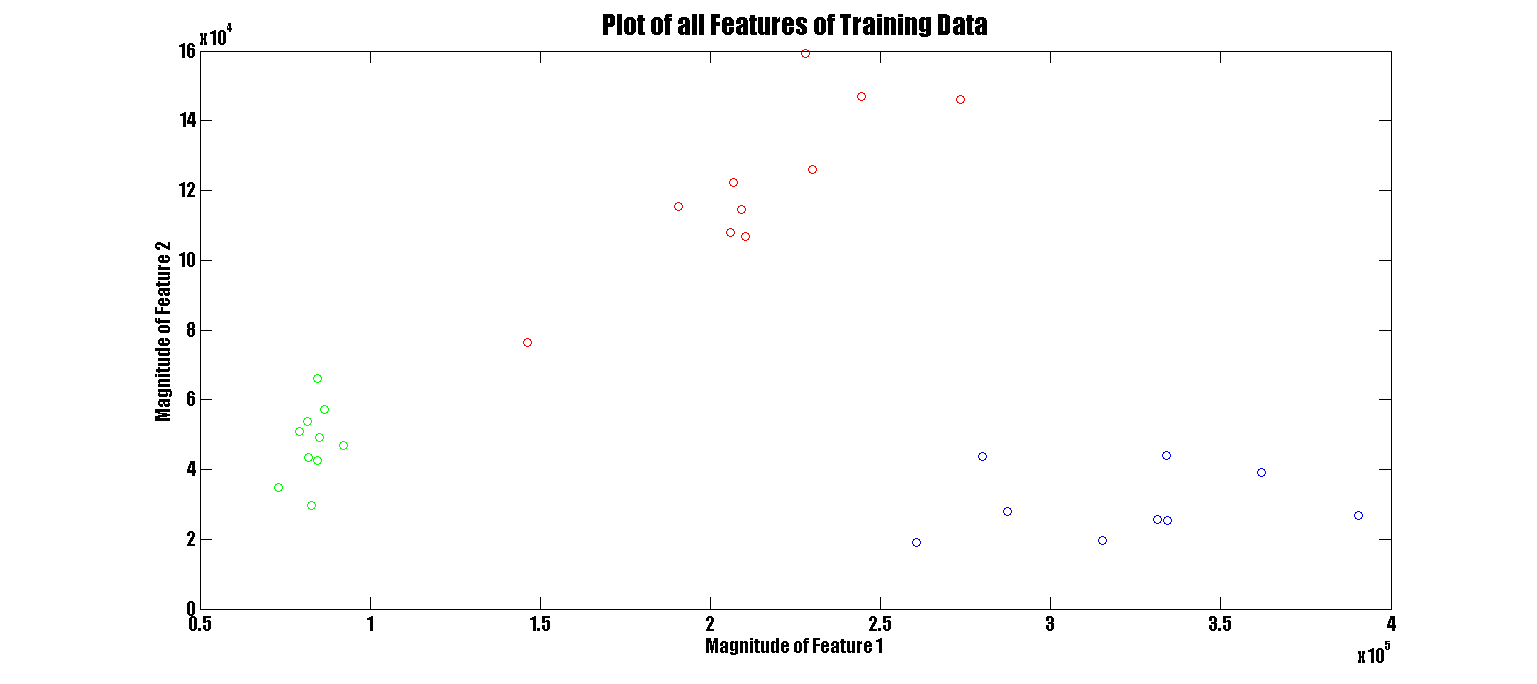
\includegraphics[width=0.5\textwidth]{plottrain.png}
\caption{\label{fig:plottrain}A Plot of the Training data features against one another. The three different clusters can be seen in green, blue and red.}
\end{figure}
In order to pick the best features to classify with, Fourier Space graphs of all three letters have to be plotted, and a combination area where the three letters differ in magnitude has to be picked, in order to allow the difference between the three letters to be shown easily. The features that were chosen were (1:180, 300:330) and (250:350, 220:265), as they separate the classes more than other values. The first was chosen as it has a high frequency when there it is used on a T, but with an S and a V it is low. The second was chosen as it has a higher frequency with an S, but low again with a V, thus splitting the classes. 
%Explain the features chosen and why you chose them
%Show graph of features plotted
\section{Classifying the Training Data}
%Explain a classifier in one sentence
A classifier is an algorithm that can be implemented to separate a dataset given a set of features. One of the tasks that was set was to implement a classifier for the training data, and plot the results on a graph.
\subsection{Classifier}
%Explain your classifiers - training and test data
In order to classify the data points, an algorithm first needed to be chosen. It was specified that a Nearest Neighbour Classifier had to be used. A Nearest Neighbour Classifier uses the neighbours of a point to create the clusters, by calculating the distance to all neighbours, and classifying the point to the same cluster as whichever neighbour has the lowest distance. In order to classify the training data provided, the Agglomerative Hierarchical Clustering method is used. 
\newline
Agglomerative Hierarchical clustering works by first setting each data point as its own cluster. It then calculates the Euclidean distance between each of the points. The algorithm then takes the two points with the lowest distance between them, and joins them in to one cluster. It then repeats, joining clusters together until there is only one singular cluster, or it can be stopped at a specified number of clusters \cite{Hierarchical Clustering}. 
\subsection{Results}
%Insert graph
\begin{figure}[H]
\centering
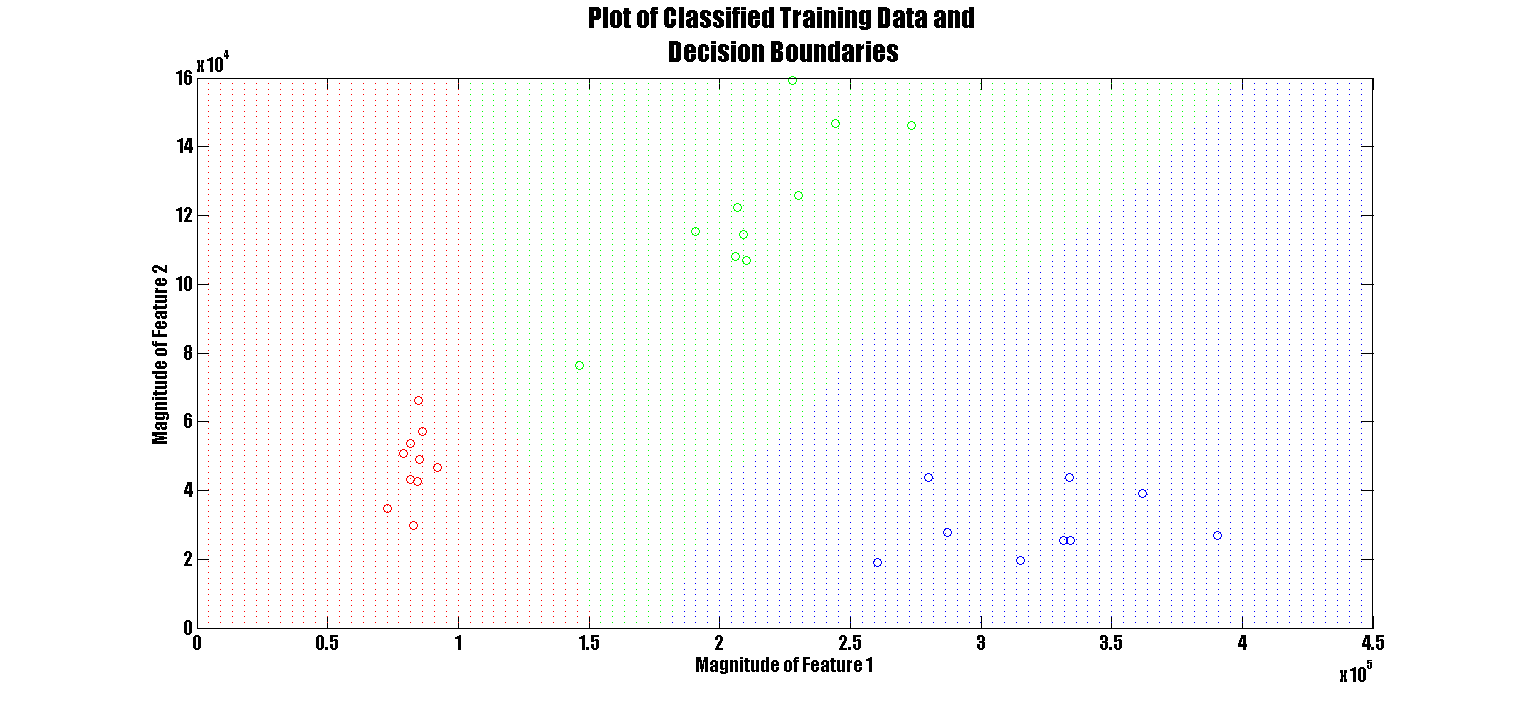
\includegraphics[width=0.5\textwidth]{plottrainclass.png}
\caption{\label{fig:plottrainclass}A Plot of the Training data features against one another, classified by Agglomerative Hierarchical Clustering. The three different clusters can be seen in green, blue and red. The decision boundaries can also be seen in these colours.}
\end{figure}
As can be seen from Figure \ref{fig:plottrainclass}, all of the data points are classified correctly to the letter they belong to. The decision boundaries can also be seen, where the red, green and blue areas meet. 
\section{Classifying Test Data}
In order to test that the training data was classified correctly, test data needed to be created and classified, in order to see how accurately the training data clusters are. 
\subsection{Data Creation}
%Explain how the data was created
The test data is created by making a 640x400 GIF, and drawing one of the letters on it. The image has to be in black and white, as the magnitudes of the Fourier Space is too high if the image is in colour or greyscale. 
%Show examples of created data
\subsection{Classifier}
%Explain the classifier that was implemented
The classifier that was implemented to classify the test data is a nearest neighbour classifier. First, it calculates the distance between all of the test data points and every training data point. It then takes the training data point with the smallest distance from the test data point, and assigns the test data point to the same cluster as the training point. It does this for all test data, until they are all clustered.
\subsection{Results}
%Explain how the data was classified
\begin{figure}[H]
\centering
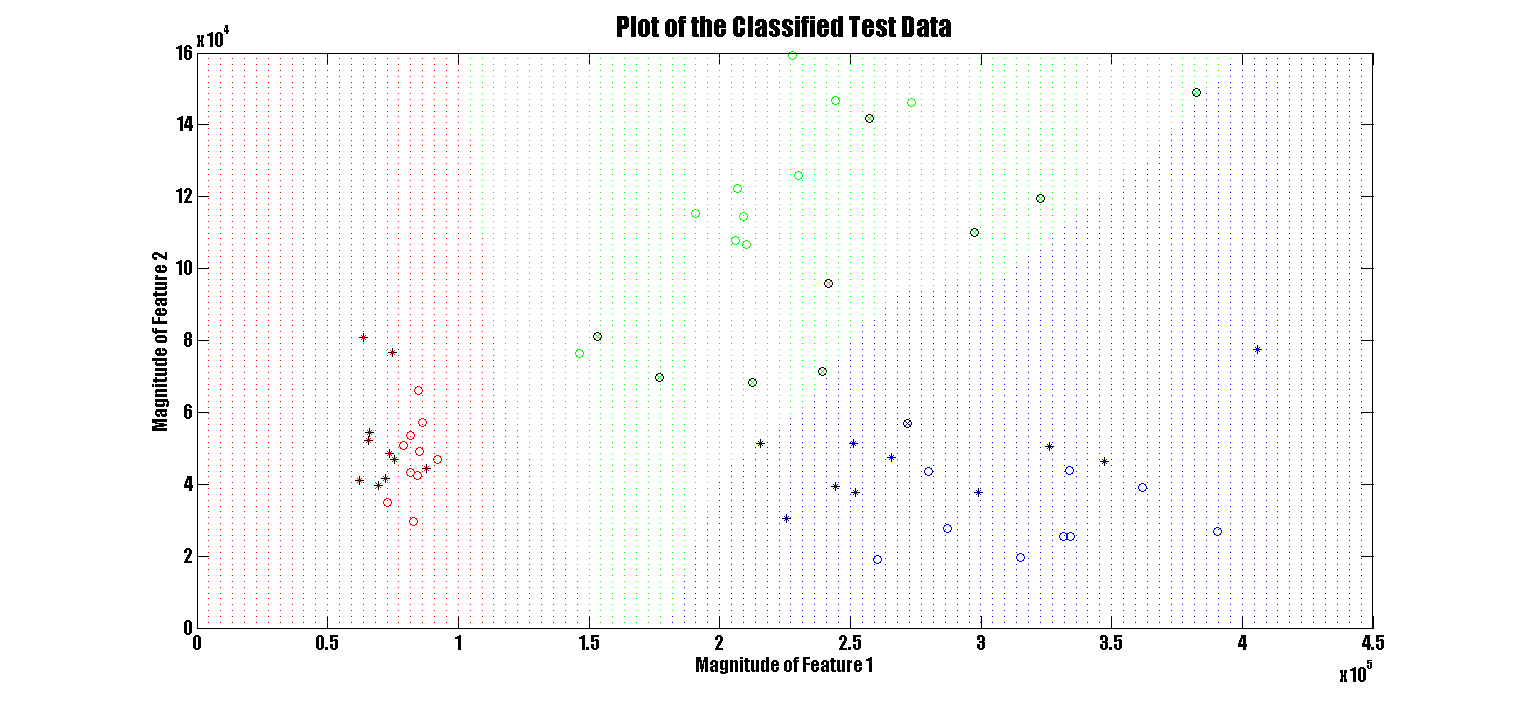
\includegraphics[width=0.5\textwidth]{plottest.png}
\caption{\label{fig:plottest}A Plot of the Test data features against one another. The three different clusters can be seen in green, blue and red.The different letters are shown by different shaped black symbols.}
\end{figure}
The three sets of test data were classified fairly well, with only one outlier, as can be seen in Figure \ref{fig:plottest}. The V's (shown in red) were classified the best, as the points are well within the cluster. The T's (in blue) were not classified quite as well, as one is very near the decision boundary, but it is within the T cluster. The S's were classified okay, but there is one S that has been classified as a T, which could be because it had a high magnitude frequency in the area of the feature that was chosen to classify T's. 
%Show results of the classification
\section{Classifying A and B}
In order to test out the classifiers to see what other behaviour it exhibits, it is possible to see how it classifies other letters as S's, T's or V's. In order to test this, an A and a B were classified as either an S, a T or a V.
\begin{figure}[H]
\centering
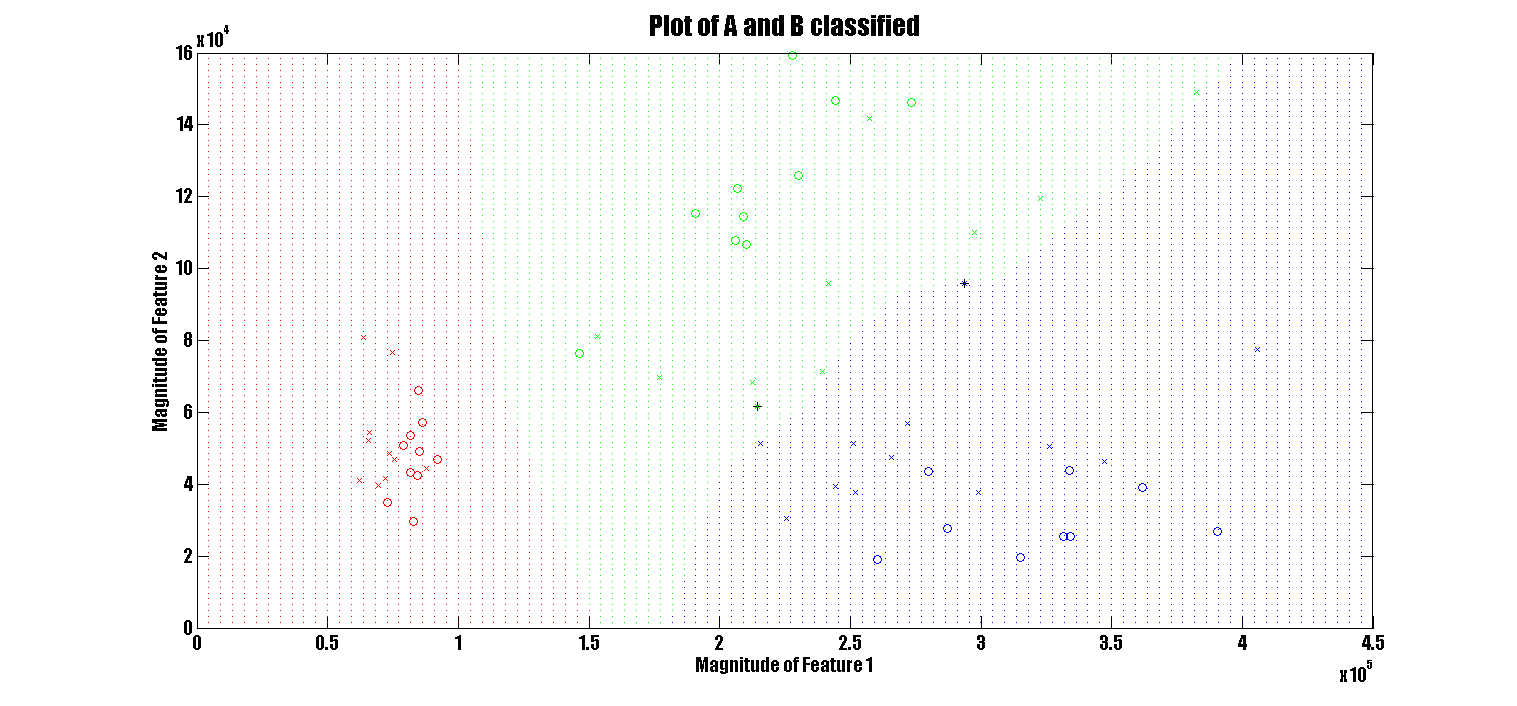
\includegraphics[width=0.5\textwidth]{plotAB.png}
\caption{\label{fig:plotAB}A Plot of the A and B images. The three different clusters can be seen in green, blue and red. The different letters are shown by different shaped black symbols.}
\end{figure}
As can be seen from Figure \ref{fig:plotAB}, the B is classified as a T and the A as an S. This is because the B has a straight line that the classifier thinks is the line from a T, and the A has a horizontal and a nearly vertical line like an S. 
\section{Alternative Classifier}
In order to test the accuracy of the Nearest Neighbour Classifier, another classifier is implemented. This classifier is a nearest centroid classifier, and the algorithm that is used to classify the training data is the K-Means algorithm.
\newline
The K-Means Clustering algorithm is one that is commonly used in data analysis. This algorithm works by taking a given number of clusters, and creating a random value, known as the centroid for each. A more accurate centroid is found for each cluster by calculating the distance between that cluster's centroid and each point. The next centroid is taken to be the mean of the points classified to it. The algorithm is then run again with the new centroid. The final centroid is taken to be the point the algorithm converges to. 
\begin{figure}[H]
\centering
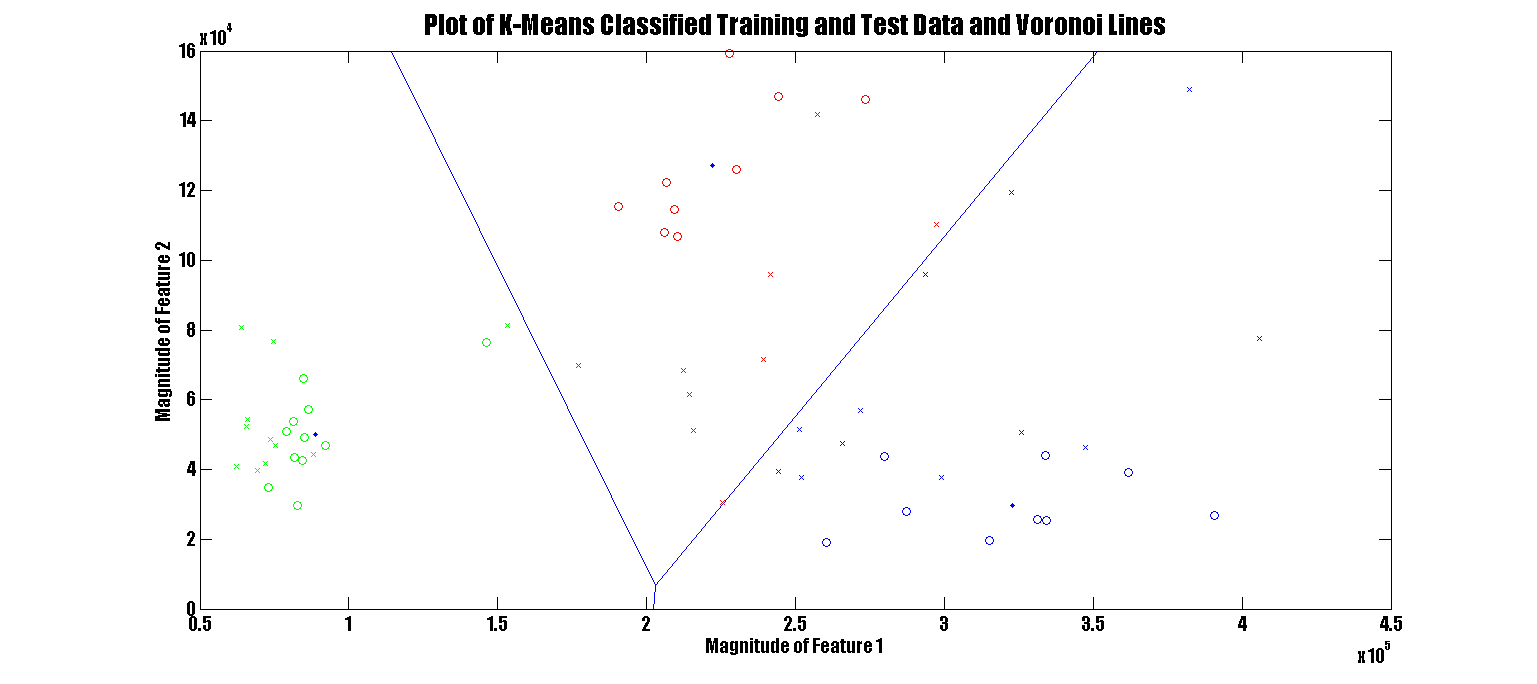
\includegraphics[width=0.5\textwidth]{plotkmeans.png}
\caption{\label{fig:plotkmeans}A Plot of the Training and Test data features against one another, classified by K-Means. The three different clusters can be seen in green, blue and red.}
\end{figure}
As can be seen from the differences between Figure \ref{fig:plotkmeans} and Figure \ref{plottrainclass}, the training data for the V's (in green) are classified correctly, as are the training data for the T's. There is one outlier in the training data for the S's, which is because the nearest centroid the this point is the centroid in the V's. The test data on the other hand isn't classified well, with some of the S's being classified as T's and vice versa. One S is also classified as a V. The errors in classification of this data shows that the nearest neighbour classification method works better for this kind of data than the nearest centroid. 
\begin{thebibliography}{1}

\bibitem{FFT}R. Fisher, S. Perkins, A. Walker and E. Wolfart. (2003), Image Transforms - Fourier Transform, url{http://homepages.inf.ed.ac.uk/rbf/HIPR2/fourier.htm}, [viewed 03/05/2014].

\bibitem{Hierarchical Clustering} Gan, G, Ma, C, Wu, J (2007). {\em Data Clustering Theory, Algorithms, and Applications}. p109-149.

\end{thebibliography}
\end{document}